\resetCUC

%1
\stepUserCase
\subsection{\valueUserCase - Visualizzazione contenuti informativi}
\labelUserCase
\begin{itemize}
    \item \textbf{Attore Primario:} cliente generico;
    \item \textbf{Descrizione:} il cliente vuole accedere alle informazioni riguardanti la piattaforma e il venditore;
    \item \textbf{Precondizione:} il cliente non sta visualizzando alcuna informazione della piattaforma;
    \item \textbf{Postcondizione:} il cliente visualizza le informazioni relative alla pagina scelta;
    \item \textbf{Scenario principale:}
          \begin{enumerate}
              \item il cliente si collega alla piattaforma e naviga fino alla pagina scelta.
          \end{enumerate}
\end{itemize}

%2
\stepUserCase
\subsection{\valueUserCase - Scelta categoria}
\labelUserCase
\begin{itemize}
    \item \textbf{Attore Primario:} cliente generico;
    \item \textbf{Descrizione:} il cliente vuole visualizzare tutti i prodotti riguardanti una determinata categoria;
    \item \textbf{Precondizione:} il cliente si trova in una pagina dove la scelta di categoria è permessa;
    \item \textbf{Input:} seleziona una categoria;
    \item \textbf{Postcondizione:} il cliente visualizza tutti i prodotti relativi alla categoria selezionata;
    \item \textbf{Scenario principale:}
          \begin{enumerate}
              \item il cliente entra in una pagina dove è presente la scelta di una categoria;
              \item seleziona una categoria;
              \item viene reindirizzato ad una pagina di visualizzazione prodotto (PLP) e visualizza i prodotti desiderati (\hyperref[UC4]{UC4}).
          \end{enumerate}
\end{itemize}

%3
\stepUserCase
\subsection{\valueUserCase - Ricerca}
\labelUserCase
\begin{itemize}
    \item \textbf{Attore Primario:} cliente generico;
    \item \textbf{Descrizione:} il cliente vuole visualizzare i prodotti che contengono nel nome prodotto una determinata parola;
    \item \textbf{Precondizione:} il cliente si trova in una pagina dove funzione di ricerca è permessa;
    \item \textbf{Input:} una stringa;
    \item \textbf{Postcondizione:} il cliente visualizza tutti i prodotti che contengono la determinata stringa nel nome;
    \item \textbf{Scenario principale:}
          \begin{enumerate}
              \item il cliente entra in una pagina dove è permessa la ricerca di un prodotto, inserisce la parola da cercare e viene reindirizzato ad una pagina di visualizzazione prodotto (PLP) e visualizza i prodotti desiderati (\hyperref[UC4]{UC4}).
          \end{enumerate}
\end{itemize}

%4
\stepUserCase
\subsection{\valueUserCase - Visualizzazione lista prodotti (PLP)}
\labelUserCase
\begin{itemize}
    \item \textbf{Attore Primario:} cliente generico;
    \item \textbf{Descrizione:} questa pagina visualizza tutti i prodotti che corrispondono ad una categoria o che corrispondono ad una parola cercata;
    \item \textbf{Precondizione:} il cliente sceglie uno dei due modi per accedere alla PLP (\hyperref[UC2]{UC2} e \hyperref[UC3]{UC3});
    \item \textbf{Postcondizione:} il cliente visualizza i prodotti che corrispondono alla scelta;
    \item \textbf{Scenario principale:}
          \begin{enumerate}
              \item il cliente può visualizzare tutti i prodotti che corrispondono alle politiche di visualizzazione;
          \end{enumerate}
    \item \textbf{Estensioni:}
          \begin{itemize}
              \item la pagina visualizza una PLP vuota perché nessun prodotto corrisponde alle politiche di visualizzazione.
          \end{itemize}
\end{itemize}

%4.1
\stepsubUserCase
\subsubsection{\valuesubUserCase - Filtri}
\labelsubUserCase
\begin{itemize}
    \item \textbf{Attore Primario:} cliente generico;
    \item \textbf{Descrizione:} il cliente può inserire ulteriori filtri per raffinare la visualizzazione dei prodotti;
    \item \textbf{Precondizione:} il cliente si deve trovare in una PLP (\hyperref[UC4]{UC4});
    \item \textbf{Postcondizione:} il cliente visualizza i prodotti con i filtri aggiornati;
    \item \textbf{Scenario principale:}
          \begin{enumerate}
              \item il cliente seleziona il filtro;
              \item il cliente modifica il valore del filtro;
              \item il cliente visualizza i prodotti secondo le nuove politiche;
          \end{enumerate}
    \item \textbf{Specializzazioni: }
          \begin{itemize}
              \item il cliente filtra i prodotti per prezzo (\hyperref[UC4.1.1]{UC4.1.1});
              \item il cliente filtra i prodotti per categoria (\hyperref[UC4.1.2]{UC4.1.2}).
          \end{itemize}
\end{itemize}

%4.1.1
\stepsubsubUserCase
\paragraph{\valuesubsubUserCase - Inserimento filtro prezzo}
\labelsubsubUserCase
\begin{itemize}
    \item \textbf{Attore Primario:} cliente generico;
    \item \textbf{Descrizione:} questa funzionalità permette al cliente di filtrare i prodotti visualizzati per prezzo;
    \item \textbf{Precondizione:} il cliente si deve trovare in una PLP (\hyperref[UC4]{UC4});
    \item \textbf{Postcondizione:} il cliente visualizza i prodotti che corrispondono alla scelta;
    \item \textbf{Scenario principale:}
          \begin{enumerate}
              \item il cliente inserisce l'intervallo di prezzo desiderato;
              \item il cliente visualizza i prodotti che corrispondono alla scelta;
          \end{enumerate}
    \item \textbf{Estensioni:}
          \begin{itemize}
              \item la pagina visualizza una PLP vuota perché nessun prodotto corrisponde alle politiche di visualizzazione.
          \end{itemize}
\end{itemize}

%4.1.2
\stepsubsubUserCase
\paragraph{\valuesubsubUserCase - Inserimento filtro categoria}
\labelsubsubUserCase
\begin{itemize}
    \item \textbf{Attore Primario:} cliente generico;
    \item \textbf{Descrizione:} questa pagina visualizza tutti i prodotti che corrispondono ad una categoria o che corrispondono ad una parola cercata;
    \item \textbf{Precondizione:} il cliente sceglie uno dei due modi per accedere alla PLP (\hyperref[UC2]{UC2} e \hyperref[UC3]{UC3});
    \item \textbf{Postcondizione:} il cliente visualizza i prodotti che corrispondono alla scelta;
    \item \textbf{Scenario principale:}
          \begin{enumerate}
              \item il cliente inserisce una nuova categoria o modifica una nuova esistente;
              \item il cliente visualizza i prodotti che corrispondono alla scelta;
          \end{enumerate}
    \item \textbf{Estensioni:}
          \begin{itemize}
              \item la pagina visualizza una PLP vuota perché nessun prodotto corrisponde alle politiche di visualizzazione.
          \end{itemize}
\end{itemize}

%5
\stepUserCase
\subsection{\valueUserCase - Apertura dettagli prodotto}
\labelUserCase
\begin{itemize}
    \item \textbf{Attore Primario:} cliente generico;
    \item \textbf{Descrizione:} questa pagina visualizza tutti i dettagli del prodotto;
    \item \textbf{Precondizione:} il cliente deve trovarsi in una pagina dove la visualizzazione dei dettagli del prodotto sia permessa;
    \item \textbf{Postcondizione:} il cliente visualizza tutti i dettagli del prodotto;
    \item \textbf{Scenario principale:}
          \begin{enumerate}
              \item il cliente visualizza tutti i dettagli del prodotto.
          \end{enumerate}
\end{itemize}

%6
\stepUserCase
\subsection{\valueUserCase - Aggiunta prodotto al carrello}
\labelUserCase
\begin{itemize}
    \item \textbf{Attore Primario:} cliente generico;
    \item \textbf{Descrizione:} questa azione serve ad aggiungere un prodotto in vendita nel sito
          all'interno del carrello personale del cliente, specificando in quale quantità;
    \item \textbf{Precondizione:} il cliente si trova nella PDP di un prodotto;
    \item \textbf{Input:} il cliente clicca sul pulsante "aggiungi al carrello" dopo aver selezionato la quantità (di default a 1);
    \item \textbf{Postcondizione:} l'oggetto è stato inserito nel carrello nella quantità desiderata (se disponibile in magazzino);
    \item \textbf{Scenario principale:}
          \begin{enumerate}
              \item il cliente seleziona la quantità desiderata o lascia quella di default;
              \item il cliente clicca sul pulsante "aggiungi al carrello" o simile;
          \end{enumerate}
    \item \textbf{Inclusioni:}
          \begin{itemize}
              \item viene eseguito un controllo sulla quantità disponibile di quel determinato prodotto;
          \end{itemize}
    \item \textbf{Estensioni:}
          \begin{itemize}
              \item in caso la quantità disponibile sia insufficiente a soddisfare la richiesta del cliente viene visualizzato un errore.
          \end{itemize}
\end{itemize}

%7
\stepUserCase
\subsection{\valueUserCase - Gestione carrello}
\labelUserCase
\begin{itemize}
    \item \textbf{Attore Primario:} cliente generico;
    \item \textbf{Descrizione:} insieme di azioni atte alla gestione degli articoli già presenti nel carrello;
    \item \textbf{Precondizione:} il cliente sta navigando il sito web;
    \item \textbf{Input:} il cliente esegue un'operazione gestionale sul carrello;
    \item \textbf{Postcondizione:} il cliente ha eseguito operazioni gestionali sul carrello;
\end{itemize}

%7.1
\stepsubUserCase
\subsubsection{\valuesubUserCase - Visualizzazione articoli}
\labelsubUserCase
\begin{itemize}
    \item \textbf{Attore Primario:} cliente generico;
    \item \textbf{Descrizione:} scenario per la visualizzazione degli articoli nel carrello;
    \item \textbf{Precondizione:} il cliente si trova su una qualunque pagina del sito web;
    \item \textbf{Input:} il cliente preme su un pulsante dedicato all'accesso al carrello;
    \item \textbf{Postcondizione:} il cliente visualizza un resoconto di tutti i prodotti inseriti nel carrello durante
          la sessione di utilizzo corrente (se non loggato), altrimenti il carrello mantiene la consistenza
          su ogni dispositivo fino al checkout.
\end{itemize}

%7.2
\stepsubUserCase
\subsubsection{\valuesubUserCase - Variazione quantità articolo}
\labelsubUserCase
\begin{itemize}
    \item \textbf{Attore primario:} cliente generico;
    \item \textbf{Descrizione:} scenario per la variazione della quantità di un singolo articolo presente nel carrello;
    \item \textbf{Precondizione:} il cliente ha eseguito \hyperref[UC7.1]{UC7.1};
    \item \textbf{Input:} il cliente inserisce la nuova quantità desiderata per quel determinato articolo;
    \item \textbf{Postcondizione:} se la quantità desiderata è disponibile, viene aggiornato l'articolo nel carrello;
    \item \textbf{Scenario principale:}
          \begin{enumerate}
              \item il cliente seleziona la nuova quantità desiderata;
              \item il cliente conferma la scelta;
          \end{enumerate}
    \item \textbf{Inclusioni:}
          \begin{itemize}
              \item viene eseguito un controllo sulla quantità disponibile di quel determinato prodotto;
          \end{itemize}
    \item \textbf{Estensioni:}
          \begin{itemize}
              \item in caso la quantità disponibile sia insufficiente a soddisfare la richiesta del cliente viene visualizzato un errore.
          \end{itemize}
\end{itemize}

%7.3
\stepsubUserCase
\subsubsection{\valuesubUserCase - Rimozione articolo}
\labelsubUserCase
\begin{itemize}
    \item \textbf{Attore Primario:} cliente generico;
    \item \textbf{Descrizione:} scenario per la rimozione di un articolo dal carrello;
    \item \textbf{Precondizione:} il cliente ha eseguito \hyperref[UC7.1]{UC7.1};
    \item \textbf{Input:} il cliente preme su un pulsante dedicato alla rimozione di un determinato articolo dal carrello;
    \item \textbf{Postcondizione:} l'articolo selezionato non è più presente nel carrello.
\end{itemize}

%8
\stepUserCase
\subsection{\valueUserCase - Checkout}
\labelUserCase
\begin{figure}[H]
    \centering
    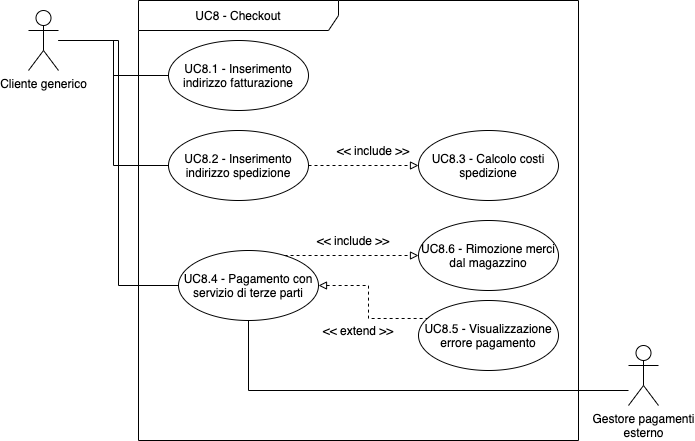
\includegraphics[width=\linewidth]{res/images/UC/UC8.png}
    \caption{Diagramma che descrive UC8 - Checkout}
\end{figure}
\begin{itemize}
    \item \textbf{Attore Primario:} cliente generico;
    \item \textbf{Descrizione:} caso d'uso per l'acquisto dei prodotti inseriti nel carrello;
    \item \textbf{Precondizione:} il cliente ha eseguito \hyperref[UC7.1]{UC7.1} e il suo carrello contiene almeno un articolo;
    \item \textbf{Input:} il cliente preme sul pulsante per avviare il checkout;
    \item \textbf{Postcondizione:} viene emesso un ordine contenente gli articoli precedentemente inseriti nel carrello. Vengono quindi rimossi dal magazzino;
    \item \textbf{Scenario principale:}
          \begin{enumerate}
              \item il cliente preme sul pulsante per avviare il checkout;
              \item inserisce gli indirizzi di fatturazione e spedizione (\hyperref[UC8.1]{UC8.1} - \hyperref[UC8.2]{8.2});
              \item vengono aggiunti i costi della spedizione all'importo totale(\hyperref[UC8.3]{UC8.3}), definiti come importo fisso;
              \item si effettua il pagamento (\hyperref[UC8.4]{UC8.4});
              \item l'ordine è stato emesso e contrassegnato come pagato;
          \end{enumerate}
    \item \textbf{Estensioni:}
          \begin{itemize}
              \item in caso di fallimento del pagamento l'ordine non viene emesso, è necessario quindi riprovare il pagamento e viene visualizzato un errore (\hyperref[UC8.6]{UC8.6});
              \item il cliente decide di annullare il processo di checkout premendo l'apposito pulsante (\hyperref[UC8.5]{UC8.5});
          \end{itemize}
\end{itemize}

%8.1
\stepsubUserCase
\subsubsection{\valuesubUserCase - Inserimento indirizzo fatturazione}
\labelsubUserCase
\begin{itemize}
    \item \textbf{Attore Primario:} cliente generico;
    \item \textbf{Descrizione:} scenario per l'inserimento dell'indirizzo di fatturazione in fase di checkout;
    \item \textbf{Precondizione:} il cliente ha avviato il processo di checkout;
    \item \textbf{Input:} il cliente inserisce i dati tramite l'apposito form oppure sceglie tra quelli personali già presenti (solo se autenticato);
    \item \textbf{Postcondizione:} il cliente procede con la fase successiva del checkout;
    \item \textbf{Scenario principale:}
          \begin{enumerate}
              \item il cliente ha 2 modi per inserire l'informazione:
                    \begin{itemize}
                        \item compilare il relativo form;
                        \item scegliere tra gli indirizzi salvati (solo se autenticato).
                    \end{itemize}
          \end{enumerate}
\end{itemize}

%8.2
\stepsubUserCase
\subsubsection{\valuesubUserCase - Inserimento indirizzo spedizione}
\labelsubUserCase
\begin{itemize}
    \item \textbf{Attore Primario:} cliente generico;
    \item \textbf{Descrizione:} scenario per l'inserimento dell'indirizzo di spedizione in fase di checkout;
    \item \textbf{Precondizione:} il cliente ha avviato il checkout;
    \item \textbf{Input:} il cliente inserisce i dati tramite l'apposito form oppure sceglie tra quelli personali già presenti (solo se autenticato);
    \item \textbf{Postcondizione:} il cliente procede con la fase successiva del checkout;
    \item \textbf{Scenario principale:}
          \begin{enumerate}
              \item il cliente ha 3 modi per inserire l'informazione:
                    \begin{itemize}
                        \item compilare il relativo form;
                        \item scegliere tra gli indirizzi salvati (solo se autenticato);
                        \item riutilizzare l'indirizzo di fatturazione precedentemente inserito.
                    \end{itemize}
          \end{enumerate}
\end{itemize}

%8.3
\stepsubUserCase
\subsubsection{\valuesubUserCase - Calcolo costi spedizione}
\labelsubUserCase
\begin{itemize}
    \item \textbf{Attore Primario:} sito EmporioLambda;
    \item \textbf{Descrizione:} scenario per il calcolo dei costi di spedizione durante il checkout;
    \item \textbf{Precondizione:} il cliente ha avviato il checkout;
    \item \textbf{Input:} il cliente inserisce l'indirizzo di spedizione;
    \item \textbf{Postcondizione:} i costi di spedizione sono stati aggiunti al totale dell'ordine da pagare
          (si aggiunge un valore fisso di 10 euro).
\end{itemize}

%8.4
\stepsubUserCase
\subsubsection{\valuesubUserCase - Pagamento con servizio di terze parti}
\labelsubUserCase
\begin{itemize}
    \item \textbf{Attore primario:} cliente generico;
    \item \textbf{Attore secondario:} gestore dei pagamenti esterno;
    \item \textbf{Descrizione:} scenario per il pagamento del totale dell'ordine mediante un gestore di pagamenti esterno a EmporioLambda;
    \item \textbf{Precondizione:} sono stati eseguiti tutti i passi precedenti del checkout, ovvero sono stati applicati i costi della spedizione al totale;
    \item \textbf{Input:} il cliente preme sul pulsante per pagare;
    \item \textbf{Postcondizione:} il pagamento è stato eseguito e l'ordine viene emesso. Vengono quindi rimosse dal magazzino le merci acquistate;
    \item \textbf{Scenario principale:}
          \begin{enumerate}
              \item il cliente premendo sul pulsante per eseguire il pagamento viene rimandato alla piattaforma esterna;
              \item esegue il pagamento interagendo con il servizio esterno;
              \item in caso di pagamento riuscito l'ordine viene emesso e le merci acquistate vengono rimosse dal magazzino (\hyperref[UC8.6]{UC8.6});
          \end{enumerate}
    \item \textbf{Estensioni:}
          \begin{itemize}
              \item in caso di pagamento fallito viene visualizzato un errore (\hyperref[UC8.5]{UC8.5}) e si offre la possibilità di riprovare premendo di nuovo sul tasto per eseguire il pagamento.
          \end{itemize}
\end{itemize}

%8.5
\stepsubUserCase
\subsubsection{\valuesubUserCase - Visualizzazione errore pagamento}
\labelsubUserCase
\begin{itemize}
    \item \textbf{Attore primario:} sito EmporioLambda;
    \item \textbf{Descrizione:} scenario per la visualizzazione di un errore dovuto al fallimento di un pagamento in fase di checkout dell'ordine;
    \item \textbf{Precondizione:} il cliente sta eseguendo il checkout dell'ordine;
    \item \textbf{Input:} il gestore esterno dei pagamenti restituisce lo stato di fallimento del pagamento;
    \item \textbf{Postcondizione:} viene visualizzato a video un messaggio che indica il fallimento del pagamento e si ritorna in condizioni di poter ritentare il pagamento.
\end{itemize}

%8.6
\stepsubUserCase
\subsubsection{\valuesubUserCase - Rimozione merci dal magazzino}
\labelsubUserCase
\begin{itemize}
    \item \textbf{Attore primario:} sito EmporioLambda;
    \item \textbf{Descrizione:} scenario per la rimozione delle merci acquistate dal magazzino;
    \item \textbf{Precondizione:} il cliente esegue sta eseguendo il checkout dell'ordine;
    \item \textbf{Input:} il gestore dei pagamenti esterno indica un successo del pagamento;
    \item \textbf{Postcondizione:} le merci acquistate vengono rimosse dal magazzino secondo i quantitativi specificati nell'ordine.
\end{itemize}

%9
\stepUserCase
\subsection{\valueUserCase - Login cliente}
\labelUserCase
\begin{itemize}
    \item \textbf{Attore primario:} cliente non autenticato;
    \item \textbf{Attore secondario:} gestore delle credenziali esterno;
    \item \textbf{Descrizione:} caso d'uso per l'autenticazione del cliente;
    \item \textbf{Precondizione:} il cliente non si è ancora autenticato nell'applicazione;
    \item \textbf{Input:} il cliente inserisce ed invia i dati per il login;
    \item \textbf{Postcondizione:} il cliente è autenticato;
    \item \textbf{Scenario principale:}
          \begin{enumerate}
              \item il cliente inserisce i dati di login (es. username e password);
              \item invia i dati inseriti;
              \item i dati vengono verificati dal gestire esterno;
              \item se i dati sono corretti e identificato un profilo utente il cliente è autenticato con questo profilo;
          \end{enumerate}
    \item \textbf{Estensioni:}
          \begin{enumerate}
              \item il gestore delle credenziali restituisce un errore indicante che i dati inseriti sono errati;
              \item viene quindi chiesto di reinserire le credenziali, contestualmente si visualizza un messaggio di errore.
          \end{enumerate}
\end{itemize}

%10
\stepUserCase
\subsection{\valueUserCase - Registrazione cliente}
\labelUserCase
\begin{itemize}
    \item \textbf{Attore primario:} cliente non autenticato;
    \item \textbf{Attore secondario:} gestore delle credenziali esterno;
    \item \textbf{Descrizione:} caso d'uso per la registrazione di un nuovo cliente;
    \item \textbf{Precondizione:} il cliente non si è ancora autenticato nell'applicazione;
    \item \textbf{Input:} il cliente inserisce ed invia i dati per la registrazione;
    \item \textbf{Postcondizione:} il cliente è autenticato con il nuovo profilo appena inserito nel sistema;
    \item \textbf{Scenario principale:}
          \begin{enumerate}
              \item il cliente inserisce l'email, la quale verrà utilizzata per contattarlo e per identificare univocamente l'utente nel sistema;
              \item il cliente reinserisce l'email per conferma;
              \item il cliente inserisce una password che rispetti i requisiti minimi di sicurezza;
              \item il cliente reinserisce la stessa password per conferma.
              \item i dati vengono inviati al servizio di terze parti per la gestione dei dati di login;
              \item arriva un'email al cliente contenente un link per la verifica all'indirizzo indicato;
              \item il cliente deve premere su quel link per attivare l'account entro una finestra di tempo limitata.
          \end{enumerate}
    \item \textbf{Estensioni:} la registrazione fallisce se:
          \begin{itemize}
              \item nel sistema esiste già un cliente con la stessa email;
              \item le due email inserite non corrispondono;
              \item le due password inserite non corrispondono;
              \item il cliente non preme il link di verifica inviato alla sua casella di posta.
          \end{itemize}
\end{itemize}

%11
\stepUserCase
\subsection{\valueUserCase - Reimpostazione password cliente}
\labelUserCase
\begin{itemize}
    \item \textbf{Attore primario:} cliente non autenticato;
    \item \textbf{Attore secondario:} gestore delle credenziali esterno;
    \item \textbf{Descrizione:} caso d'uso per la reimpostazione della password, utile quando il cliente la dimentica;
    \item \textbf{Precondizione:} il cliente non si è ancora autenticato nell'applicazione e si trova nella pagina di login;
    \item \textbf{Input:} il cliente si accorge di aver dimenticato la password di accesso e preme sul pulsante per la reimpostazione;
    \item \textbf{Postcondizione:} il cliente ha modificato la sua password e può effettuare il login;
    \item \textbf{Scenario principale:}
          \begin{enumerate}
              \item il cliente chiede la reimpostazione della password;
              \item riceve tramite email un link per la reimpostazione valido entro un certo limite di tempo;
              \item preme sul link e viene portato su una pagina per l'inserimento della password;
              \item inserisce la nuova password;
              \item reinserisce la password per conferma;
              \item invia i dati inseriti al gestore delle credenziali.
          \end{enumerate}
    \item \textbf{Estensioni:} la reimpostazione della password fallisce se:
          \begin{itemize}
              \item le password inserite non corrispondono;
              \item la nuova password non rispetta i requisiti minimi di sicurezza.
          \end{itemize}
\end{itemize}

%12
\stepUserCase
\subsection{\valueUserCase - Amministrazione account}
\labelUserCase
\begin{figure}[H]
    \centering
    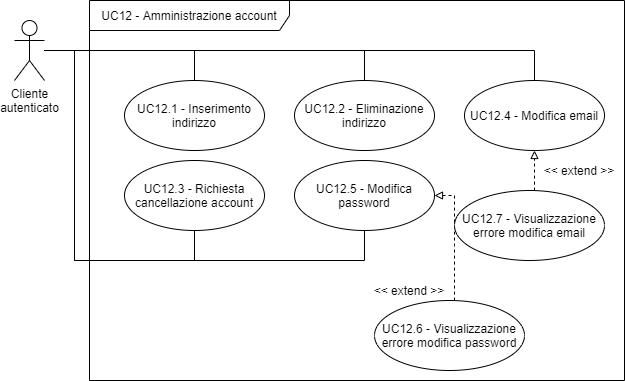
\includegraphics[width=\linewidth]{res/images/UC/UC12.png}
    \caption{Diagramma che descrive UC12 - Amministrazione account}
\end{figure}
\begin{itemize}
    \item \textbf{Attore Primario:} cliente autenticato;
    \item \textbf{Descrizione:} caso d'uso per la gestione del profilo utente di un cliente;
    \item \textbf{Precondizione:} il cliente ha eseguito il login (\hyperref[UC9]{UC9}) e si trova sulla pagina per la gestione del profilo;
    \item \textbf{Input:} il cliente avvia un'operazione di gestione profilo;
    \item \textbf{Postcondizione:} il cliente ha modificato il suo profilo o richiesto la modifica al venditore.
\end{itemize}

%12.1
\stepsubUserCase
\subsubsection{\valuesubUserCase - Inserimento indirizzo}
\labelsubUserCase
\begin{itemize}
    \item \textbf{Attore primario:} cliente autenticato;
    \item \textbf{Descrizione:} scenario per l'inserimento di un nuovo indirizzo (utilizzabile per spedizione e/o fatturazione in fase di checkout);
    \item \textbf{Precondizione:} il cliente ha eseguito il login (\hyperref[UC9]{UC9}) e si trova sulla pagina per la gestione del profilo;
    \item \textbf{Input:} il cliente seleziona l'opzione per inserire un nuovo indirizzo;
    \item \textbf{Postcondizione:} nel sistema esiste l'indirizzo inserito dal cliente;
    \item \textbf{Scenario principale:}
          \begin{enumerate}
              \item il cliente compila il form per l'inserimento dell'indirizzo;
              \item il cliente invia quindi i dati.
          \end{enumerate}
\end{itemize}

%12.2
\stepsubUserCase
\subsubsection{\valuesubUserCase - Eliminazione indirizzo}
\labelsubUserCase
\begin{itemize}
    \item \textbf{Attore primario:} cliente autenticato;
    \item \textbf{Descrizione:} scenario per l'eliminazione di un indirizzo precedentemente inserito;
    \item \textbf{Precondizione:} il cliente ha eseguito il login (\hyperref[UC9]{UC9}) e si trova sulla pagina per la gestione del profilo;
    \item \textbf{Input:} il cliente seleziona l'opzione per eliminare un indirizzo;
    \item \textbf{Postcondizione:} nel sistema non esiste più l'indirizzo rimosso.
\end{itemize}

%12.3
\stepsubUserCase
\subsubsection{\valuesubUserCase - Richiesta cancellazione account}
\labelsubUserCase
\begin{itemize}
    \item \textbf{Attore primario:} cliente autenticato;
    \item \textbf{Descrizione:} scenario per la richiesta di cancellazione del profilo cliente al venditore;
    \item \textbf{Precondizione:} il cliente ha eseguito il login (\hyperref[UC9]{UC9}) e si trova sulla pagina per la gestione del profilo;
    \item \textbf{Input:} il cliente sceglie l'opzione per aprire un ticket di assistenza e richiedere la cancellazione dell'account;
    \item \textbf{Postcondizione:} è stato aperto un ticket di assistenza nella piattaforma, il venditore quindi provvederà a gestirlo opportunamente.
\end{itemize}

%12.4
\stepsubUserCase
\subsubsection{\valuesubUserCase - Modifica email}
\labelsubUserCase
\begin{itemize}
    \item \textbf{Attore primario:} cliente autenticato;
    \item \textbf{Descrizione:} scenario per la modifica dell'email (username) dell'utente;
    \item \textbf{Precondizione:} il cliente ha eseguito il login (\hyperref[UC9]{UC9}) e si trova sulla pagina per la gestione del profilo;
    \item \textbf{Input:} il cliente sceglie l'opzione per modificare l'email che lo identifica univocamente all'interno del sito;
    \item \textbf{Postcondizione:} l'email è stata modificata con quella nuova inserita;
    \item \textbf{Scenario principale:}
          \begin{enumerate}
              \item il cliente inserisce l'email nel campo apposito;
              \item il cliente reinserisce la stessa email in un altro campo per la verifica;
              \item il cliente invia quindi i dati inseriti;
              \item si ripete il processo di verifica email spiegato nel caso d'uso della registrazione.
          \end{enumerate}
    \item \textbf{Estensioni:} la modifica dell'email fallisce se:
          \begin{itemize}
              \item i due indirizzi email non corrispondono;
              \item il nuovo indirizzo non viene verificato.
          \end{itemize}
\end{itemize}

%12.5
\stepsubUserCase
\subsubsection{\valuesubUserCase - Modifica password}
\labelsubUserCase
\begin{itemize}
    \item \textbf{Attore primario:} cliente autenticato;
    \item \textbf{Descrizione:} scenario per la modifica della password del cliente;
    \item \textbf{Precondizione:} il cliente ha eseguito il login (\hyperref[UC9]{UC9}) e si trova sulla pagina per la gestione del profilo;
    \item \textbf{Input:} il cliente seleziona l'opzione per modificare la password di accesso;
    \item \textbf{Postcondizione:} la password di accesso al sistema per quel cliente è stata modificata;
    \item \textbf{Scenario principale:}
          \begin{enumerate}
              \item il cliente inserisce la vecchia password;
              \item il cliente inserisce la nuova password;
              \item il cliente reinserisce la nuova password;
              \item il cliente invia quindi i dati inseriti.
          \end{enumerate}
    \item \textbf{Estensioni:} la modifica della password fallisce se:
          \begin{itemize}
              \item le password inserite non corrispondono;
              \item la nuova password non rispetta i requisiti minimi di sicurezza.
          \end{itemize}
\end{itemize}

%13
\stepUserCase
\subsection{\valueUserCase - Gestione ordini cliente}
\labelUserCase
\begin{itemize}
    \item \textbf{Attore Primario:} cliente autenticato;
    \item \textbf{Descrizione:} il cliente vuole accedere all'area di gestione degli ordini;
    \item \textbf{Precondizione:} il cliente è loggato nel sito;
    \item \textbf{Postcondizione:} il cliente risulta nella pagina dove è presente la lista di tutti gli ordini effettuati;
    \item \textbf{Scenario principale:}
          \begin{enumerate}
              \item il cliente entra nella pagina con la lista degli ordini;
              \item il cliente può annullare l'ordine (\hyperref[UC13.1]{UC13.1});
              \item il cliente può richiedere assistenza per un ordine (\hyperref[UC13.2]{UC13.2});
              \item il cliente può richiedere un reso (\hyperref[UC13.3]{UC13.3});
              \item il cliente può visualizzare il riepilogo di un determinato ordine (\hyperref[UC13.4]{UC13.4}).
          \end{enumerate}
\end{itemize}

%13.1
\stepsubUserCase
\subsubsection{\valuesubUserCase - Annullamento ordine}
\labelsubUserCase
\begin{itemize}
    \item \textbf{Attore Primario:} cliente autenticato;
    \item \textbf{Descrizione:} il cliente vuole annullare un ordine effettuato;
    \item \textbf{Precondizione:} il cliente deve aver effettuato un ordine e trovarsi nella sezione gestione degli ordini;
    \item \textbf{Postcondizione:} il cliente deve aver contatto il venditore per l'annullamento;
    \item \textbf{Scenario principale:}
          \begin{enumerate}
              \item il cliente sceglie ordine da annullare;
              \item il cliente viene portato al form di contatto dove sarà già precompilato il numero dell'ordine che si desidera annullare;
          \end{enumerate}
    \item \textbf{Inclusioni:}
          \begin{itemize}
              \item per annullare un ordine viene aperto il form di contatto che permette al cliente di contattare il venditore (\hyperref[UC15]{UC15}).
          \end{itemize}
\end{itemize}

%13.2
\stepsubUserCase
\subsubsection{\valuesubUserCase - Assistenza cliente}
\labelsubUserCase
\begin{itemize}
    \item \textbf{Attore Primario:} cliente autenticato;
    \item \textbf{Descrizione:} il cliente vuole contattare il venditore per un problema (errore indirizzo, domande, etc.);
    \item \textbf{Precondizione:} il cliente deve trovarsi nella pagina della gestione degli ordini e quindi aver effettuato l'ordine;
    \item \textbf{Postcondizione:} il cliente deve aver contatto il venditore per richiedere assistenza;
    \item \textbf{Scenario principale:}
          \begin{enumerate}
              \item il cliente decide di contattare l'assistenza;
              \item il cliente viene portato al form di contatto dove sarà già precompilato il numero dell'ordine al quale si desidera chiedere assistenza;
          \end{enumerate}
    \item \textbf{Inclusioni:}
          \begin{itemize}
              \item per l'assistenza su un ordine viene aperto il form di contatto che permette al cliente di contattare il venditore (\hyperref[UC15]{UC15}).
          \end{itemize}
\end{itemize}

%13.3
\stepsubUserCase
\subsubsection{\valuesubUserCase - Richiesta reso}
\labelsubUserCase
\begin{itemize}
    \item \textbf{Attore Primario:} cliente autenticato;
    \item \textbf{Descrizione:} il cliente vuole effettuare un reso di un ordine ricevuto;
    \item \textbf{Precondizione:} il cliente deve aver effettuato un ordine, averlo ricevuto, ed essere nella pagina di gestione degli ordini;
    \item \textbf{Postcondizione:} il cliente deve aver contatto il venditore per il reso;
    \item \textbf{Scenario principale:}
          \begin{enumerate}
              \item il cliente decide di effettuare un reso;
              \item il cliente viene portato al form di contatto dove sarà già precompilato il numero dell'ordine di cui si desidera effettuare il reso;
          \end{enumerate}
    \item \textbf{Inclusioni:}
          \begin{itemize}
              \item per il reso di un ordine viene aperto il form di contatto che permette al cliente di contattare il venditore (\hyperref[UC15]{UC15}).
          \end{itemize}
\end{itemize}

%13.4
\stepsubUserCase
\subsubsection{\valuesubUserCase - Riepilogo ordine}
\labelsubUserCase
\begin{itemize}
    \item \textbf{Attore Primario:} cliente autenticato;
    \item \textbf{Descrizione:} il cliente vuole visualizzare il riepilogo dell'ordine effettuato;
    \item \textbf{Precondizione:} il cliente deve aver effettuato l'ordine e trovarsi nella pagina di gestione degli ordini;
    \item \textbf{Postcondizione:} il cliente visualizza il riepilogo;
    \item \textbf{Scenario principale:}
          \begin{enumerate}
              \item il cliente decide di aprire il riepilogo dell'ordine;
              \item si apre la pagina dove è presentato il riepilogo.
          \end{enumerate}
\end{itemize}

%14
\stepUserCase
\subsection{\valueUserCase - Logout cliente}
\labelUserCase
\begin{itemize}
    \item \textbf{Attore Primario:} cliente autenticato;
    \item \textbf{Descrizione:} il cliente vuole uscire dal sito;
    \item \textbf{Precondizione:} il cliente è loggato al sito;
    \item \textbf{Postcondizione:} il cliente risulta non autenticato nel sito;
    \item \textbf{Scenario principale:}
          \begin{enumerate}
              \item il cliente effettua il logout;
              \item il cliente si ritrova nella pagina principale del sito.
          \end{enumerate}
\end{itemize}

%15
\stepUserCase
\subsection{\valueUserCase - Contatta venditore}
\labelUserCase
\begin{itemize}
    \item \textbf{Attore Primario:} cliente generico;
    \item \textbf{Descrizione:} il cliente vuole/deve contattare il venditore attraverso il form di contatto;
    \item \textbf{Precondizione:} il cliente sta navigando il sito, o arriva da \hyperref[UC13.1]{UC13.1}, \hyperref[UC13.2]{UC13.2} o \hyperref[UC13.3]{UC13.3};
    \item \textbf{Postcondizione:} il cliente riesce a contattare il venditore;
    \item \textbf{Scenario principale:}
          \begin{enumerate}
              \item il cliente ha aperto il form di contatto;
              \item il cliente compila il form;
              \item eventualmente il cliente inserisce il numero dell'ordine a cui si vuole riferire (se non giunge da \hyperref[UC13.1]{UC13.1}, \hyperref[UC13.2]{UC13.2} o \hyperref[UC13.3]{UC13.3}, in quanto viene inserito in automatico.) ;
              \item il cliente contatta con successo il venditore.
          \end{enumerate}
\end{itemize}